\begin{frame}{$p(K^-, \pi^+ \pi^-)"n"$ events}
  \begin{tabular}{cc}
    \begin{minipage}{0.3\hsize}
      \begin{figure}
        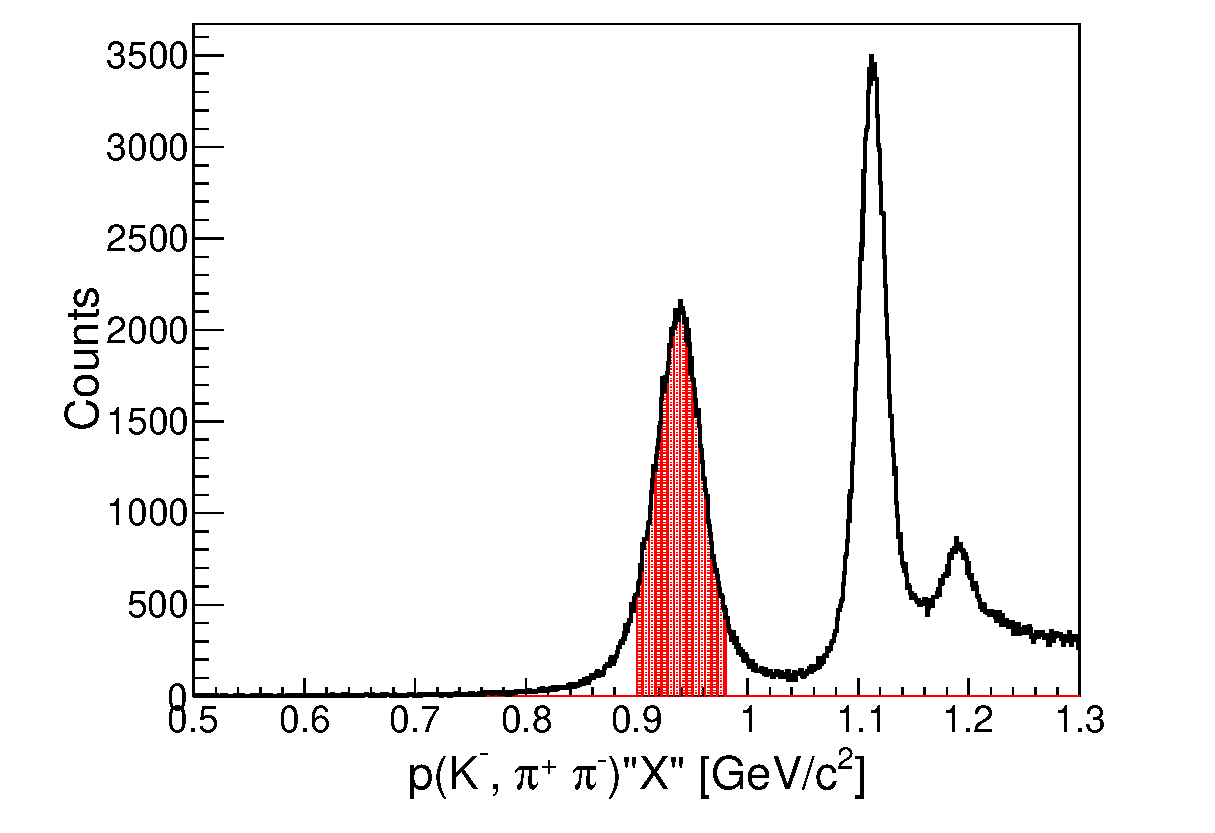
\includegraphics[width=4cm]{../pic/Run62/NC_eff/pipi_MM.eps}
      \end{figure}
    \end{minipage}

    \begin{minipage}{0.7\hsize}
      \begin{enumerate}
      \item $K^- p \rightarrow K^0 n$\\
        This reaction was selected by $\pi^+ \pi^-$ IM.
      \item $K^- p \rightarrow \pi^- \Sigma^+$
      \item $K^- p \rightarrow \pi^+ \Sigma^-$\\
        { \scriptsize
          These two reactions were rejected by $d(K^-, \pi^{\mp})"\Sigma^{\pm}"$
        }
      \end{enumerate}
    \end{minipage}
  \end{tabular}

  \begin{tabular}{cc}
    \begin{minipage}{0.5\hsize}
      \begin{figure}
        $\Sigma^{\pm}$ rejection
        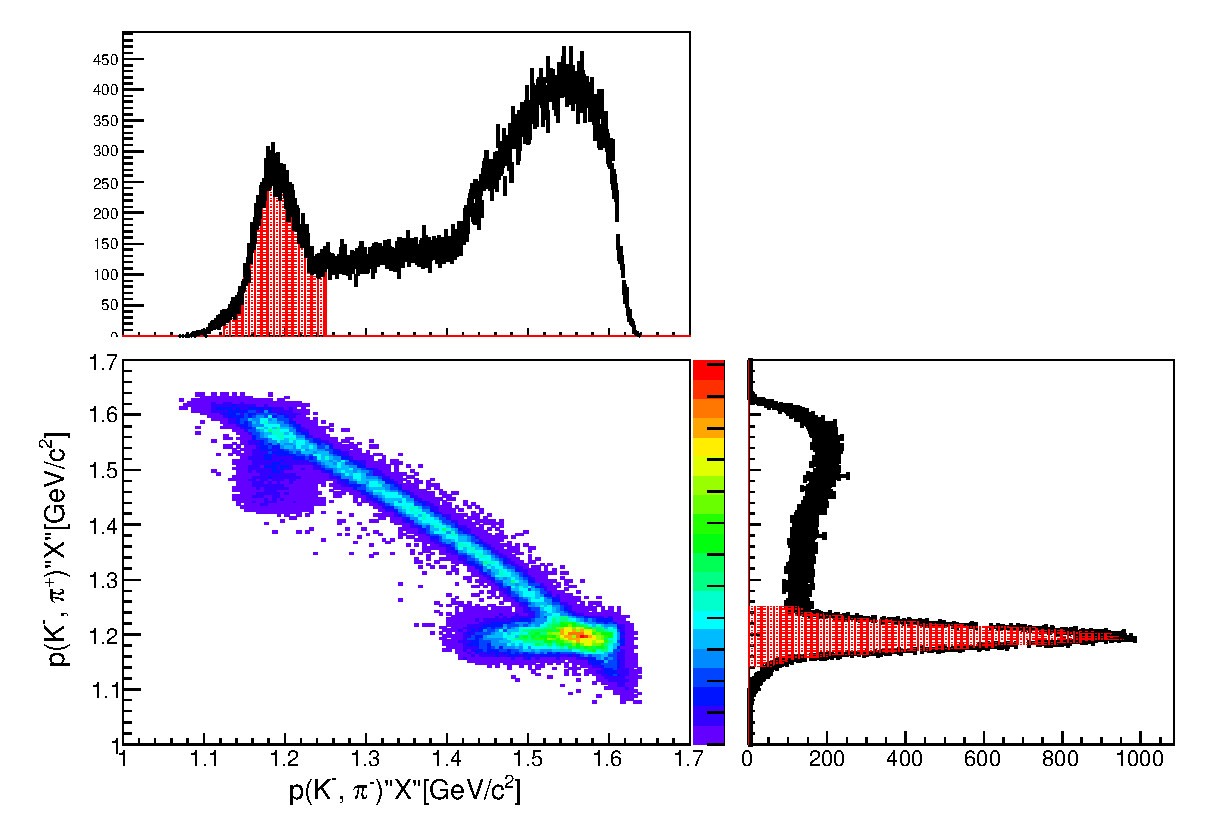
\includegraphics[width=5cm]{../pic/Run62/NC_eff/Ppim_Ppip_MM.eps}
      \end{figure}
    \end{minipage}

    \begin{minipage}{0.5\hsize}
      \begin{figure}
        $K^0$ selection
        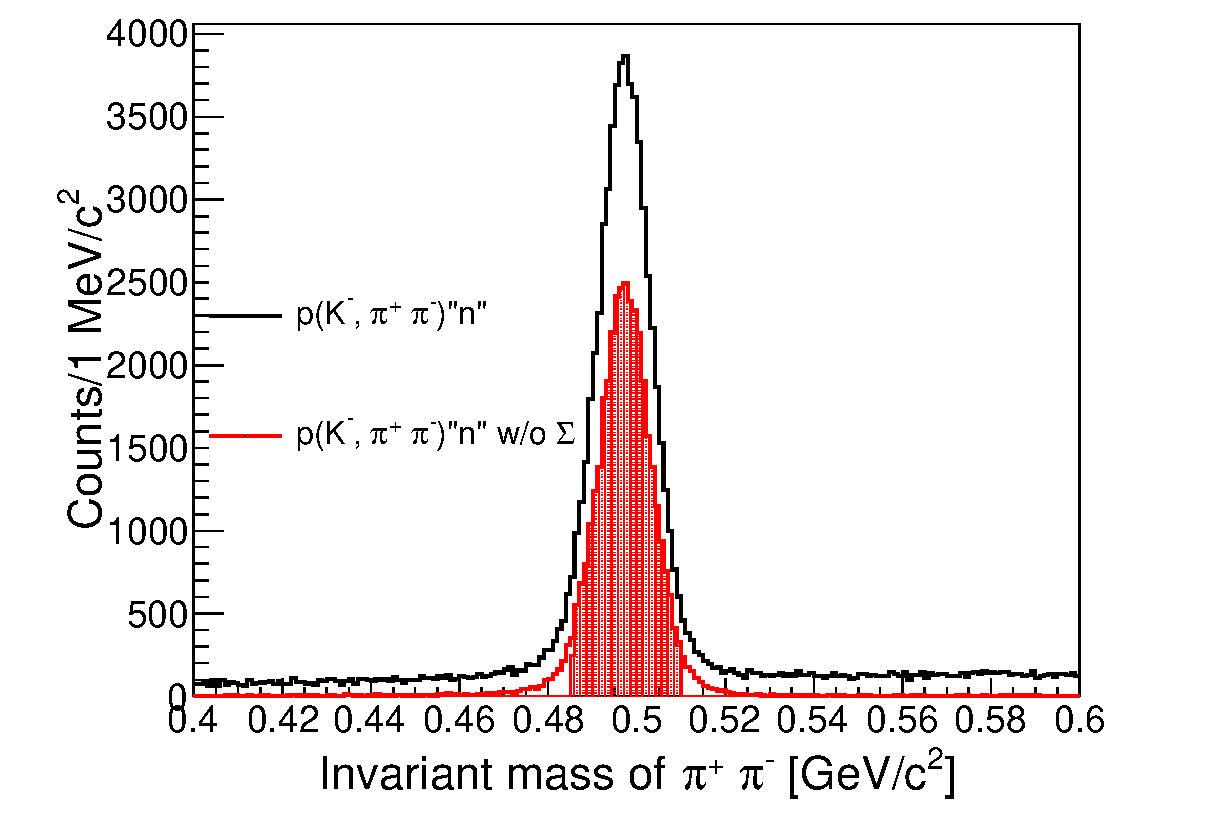
\includegraphics[width=4.5cm]{../pic/Run62/NC_eff/CDS_IM_pipi.eps}
      \end{figure}
    \end{minipage}
  \end{tabular}
\end{frame}
